%%%%%%%%%%%%%%%%%%%%%%%%%%%%%%%%%%%%%%%%%%%
%
% From a template maintained at https://github.com/jamesrobertlloyd/cbl-tikz-poster
%
% Code near the top should be fairly standard and not need to be changed
%  - except for the document class
% Code lower down is more likely to be customised
%
%%%%%%%%%%%%%%%%%%%%%%%%%%%%%%%%%%%%%%%%%%%

%%%%%%%%%%%%%%%%%%%%%%%%%%%%%%%%%%%%%%%%%%%
%
% Document class
%
% Change this if you want a different size / orientation poster etc
%
%%%%%%%%%%%%%%%%%%%%%%%%%%%%%%%%%%%%%%%%%%%

%\documentclass[landscape,a0b,final,a4resizeable]{a0poster}
\documentclass[portrait,a0b,final,a4resizeable]{a0poster}

%%%%%%%%%%%%%%%%%%%%%%%%%%%%%%%%%%%%%%%%%%%
%
% 'Basic' packages
%
% TODO - Almost certainly some are unnecessary - feel free to remove nonstandard
% packages if you think it is a good idea not to always have them
%
%%%%%%%%%%%%%%%%%%%%%%%%%%%%%%%%%%%%%%%%%%%
\usepackage{graphicx}
% \usepackage[draft]{graphicx}
\graphicspath{ {fig/} }
 \usepackage[export]{adjustbox}
 
\usepackage{todonotes}
\usepackage[inline]{enumitem}
\usepackage{bm}

\usepackage{sty/msoelch/mlmacros}
\usepackage{amsmath}
\usepackage{mathtools}
\usepackage{calc}
\usepackage{fontawesome}
\usepackage{hyperref}

%\usepackage[osf,sc]{mathpazo} % Palatino as the main font
%\linespread{1.05}\selectfont % Palatino needs some extra spacing, here 5% extra
% \usepackage[euler-digits]{eulervm} % nicer math font

% \usepackage{floatrow}
\usepackage[skip=5pt]{caption}
\usepackage{subcaption}

\usepackage[noabbrev]{cleveref}

% section spacing
\usepackage{titlesec}

\titlespacing*{\section}
{0pt}{.1\baselineskip}{.1\baselineskip}
  
% Decrease spacing between bib entries
%\setlength{\bibsep}{0pt plus 0.3ex}

\newcommand*{\B}[1]{\ifmmode\bm{#1}\else\textbf{#1}\fi}

\variables{a,b,c,g,t,o,s,v,x,z}
\variables{A,I}

\variables[app]{\alpha}
\variables[mean]{\mu}
\variables[std]{\sigma}
\variables[map]{\nu}
\variables[dparam]{\psi}

% Neil's comment function
\newcommand{\nd}[1]{\textcolor{red}{[ND: #1]}}
\newcommand{\ab}[1]{\textcolor{green}{[AB: #1]}}
\newcommand{\ak}[1]{\textcolor{blue}{[AK: #1]}}

\probdists{p,q}

\DeclarePairedDelimiter{\fences}{(}{)}
\DeclarePairedDelimiter{\norm}{\lVert}{\rVert}

%\DeclareMathOperator{\MLP}{ \mathrm{MLP} \Fences }
\newcommand{\MLP}[1]{ \mathrm{MLP} \fences{#1} }
\newcommand{\LSTM}[1]{ \mathrm{LSTM} \fences{#1} }
\newcommand{\flatten}[1]{ \mathrm{vec} \fences{#1} }

\newcommand{\reg}[1]{ \ensuremath{R} \fences{#1} }

\definecolor{darkgreen}{rgb}{0,.502,0}

\newcommand{\sidecaption}[1]% #1 = label name
{\raisebox{\abovecaptionskip}{\begin{subfigure}[t]{1.6em}
  \caption[singlelinecheck=off]{}% do not center
  \label{#1}
\end{subfigure}}\ignorespaces}

\usepackage[margin={4mm,4mm}]{geometry}
\usepackage{multicol}
\usepackage{color}
\usepackage{shadow}
\usepackage{morefloats}
\usepackage{cite}
%\usepackage[pdftex]{graphicx}
\usepackage{rotating}
\usepackage{amsmath, amsthm, amssymb, bm}
\usepackage{array}
\usepackage{nth}
\usepackage[square,numbers]{natbib}
\usepackage{booktabs}


%%%%%%%%%%%%%%%%%%%%%%%%%%%%%%%%%%%%%%%%%%%
%
% TIKZ packages and common definitions
%
% Add extra things as per your tikz needs
%
%%%%%%%%%%%%%%%%%%%%%%%%%%%%%%%%%%%%%%%%%%%

\usepackage{../common/picins}
\usepackage{tikz}
\usepackage{tabularx}
\usetikzlibrary{shapes.geometric,arrows,chains,arrows.meta,matrix,positioning,scopes,calc}
\tikzstyle{mybox} = [draw=none, rectangle]

%%%%%%%%%%%%%%%%%%%%%%%%%%%%%%%%%%%%%%%%%%%
%
% myfig
%
% \myfig - replacement for \figure
% necessary, since in multicol-environment 
% \figure won't work        
%                 
%%%%%%%%%%%%%%%%%%%%%%%%%%%%%%%%%%%%%%%%%%%

\newcommand{\myfig}[3][0]{
\begin{center}
  \vspace{1.5cm}
  \includegraphics[width=#3\hsize,angle=#1]{#2}
  \nobreak\medskip
\end{center}}

%%%%%%%%%%%%%%%%%%%%%%%%%%%%%%%%%%%%%%%%%%%
%
% mycaption                
%
% \mycaption - replacement for \caption
% necessary, since in multicol-environment \figure and
% therefore \caption won't work
%
%%%%%%%%%%%%%%%%%%%%%%%%%%%%%%%%%%%%%%%%%%%

%\newcounter{figure}
\setcounter{figure}{1}
\newcommand{\mycaption}[1]{
  \vspace{0.5cm}
  \begin{quote}
    {{\sc Figure} \arabic{figure}: #1}
  \end{quote}
  \vspace{1cm}
  \stepcounter{figure}
}

%%%%%%%%%%%%%%%%%%%%%%%%%%%%%%%%%%%%%%%%%%%
%
% Some standard colours
%
%%%%%%%%%%%%%%%%%%%%%%%%%%%%%%%%%%%%%%%%%%%

%\definecolor{oriblue}{cmyk}{1., .8, 0., .6}
\definecolor{oriblue}{RGB}{0, 33, 71}
\definecolor{camlightblue}{rgb}{0.601 , 0.8, 1}
\definecolor{camdarkblue}{rgb}{0, 0.203, 0.402}
\definecolor{camred}{rgb}{1, 0.203, 0}
\definecolor{camyellow}{rgb}{1, 0.8, 0}
\definecolor{lightblue}{rgb}{0, 0, 0.80}
\definecolor{white}{rgb}{1, 1, 1}
\definecolor{whiteblue}{rgb}{0.80, 0.80, 1}

%%%%%%%%%%%%%%%%%%%%%%%%%%%%%%%%%%%%%%%%%%%
%
% Some look and feel definitions
%
%%%%%%%%%%%%%%%%%%%%%%%%%%%%%%%%%%%%%%%%%%%

\setlength{\columnsep}{0.03\textwidth}
\setlength{\columnseprule}{0.0018\textwidth}
\setlength{\parindent}{0.0cm}

%%%%%%%%%%%%%%%%%%%%%%%%%%%%%%%%%%%%%%%%%%%
%
% \ - replacement for \section*
% 
% Puts a pretty box around some text
% TODO - any other thoughts for what this box should look like
%
%%%%%%%%%%%%%%%%%%%%%%%%%%%%%%%%%%%%%%%%%%%

\tikzstyle{mysection} = [rectangle, 
									draw=none, 
									shade, 
									outer color=oriblue,
									inner color=oriblue,
									text width=0.965\columnwidth,
									text centered,
									rounded corners=20pt,
									minimum height=0.11\columnwidth]

\newcommand{\mysection}[1]
{
\begin{center}
  \begin{tikzpicture}
    \node[mysection] {\textcolor{white}{\sffamily\bfseries\LARGE#1}};
  \end{tikzpicture}
\end{center}
}

%%%%%%%%%%%%%%%%%%%%%%%%%%%%%%%%%%%%%%%%%%%
%
% Set the font
%
% TODO - Not sure what a canonical choice is - feel free to modify
%
%%%%%%%%%%%%%%%%%%%%%%%%%%%%%%%%%%%%%%%%%%%

\renewcommand{\familydefault}{cmss}
\sffamily

%%%%%%%%%%%%%%%%%%%%%%%%%%%%%%%%%%%%%%%%%%%
%
% Poster environment
%
% Centres everything and can be used to define the width of the content
%
%%%%%%%%%%%%%%%%%%%%%%%%%%%%%%%%%%%%%%%%%%%

\newenvironment{poster}{
  \begin{center}
  \begin{minipage}[c]{0.96\textwidth}
}{
  \end{minipage} 
  \end{center}
}

%%%%%%%%%%%%%%%%%%%%%%%%%%%%%%%%%%%%%%%%%%%
%
% This is probably a good place to put content specific packages and definitions
%
%%%%%%%%%%%%%%%%%%%%%%%%%%%%%%%%%%%%%%%%%%%

\newtheorem{thm}{Theorem}%[section]
\newtheorem{lem}[thm]{Lemma}
\newtheorem{prop}[thm]{Proposition}
\newtheorem{cor}[thm]{Corollary}

\newtheorem*{theorem*}{Theorem}

\theoremstyle{definition}
\newtheorem*{definition*}{Definition}
\newtheorem{definition}[thm]{Definition}%[section]
\newtheorem{conj}{Conjecture}[section]
\newtheorem{exmp}{Example}[section]
\newtheorem{rem}[thm]{Remark}

\theoremstyle{remark}
%\newtheorem{rem}{Remark}
\newtheorem{note}{Note}
\newtheorem{case}{Case}

\newcommand{\eqd}{\overset{\,_{\!d}}{=}}
\newcommand{\defn}[1]{\emph{#1}}

\newcommand{\Law}{\mathcal{L}}

\def\given{\,|\,}

\def\SGinf{\mathbb{S}_{\infty}}

\newcommand{\NonNegInts}{\mathbb{Z}_+}
\newcommand{\Nats}{\mathbb{N}}
\newcommand{\Rationals}{\mathbb{Q}}
\newcommand{\Reals}{\mathbb{R}}

\newcommand{\as}{\textrm{a.s.}}

\def\[#1\]{\begin{align}#1\end{align}}
\newcommand{\defas}{:=}

\newcommand{\Normal}{\mathcal{N}}
\newcommand{\dist}{\ \sim\ }

\newcommand{\kernel}{\kappa}
\newcommand{\kernelmatrix}{K}
\newcommand{\scalefactor}{s}
\newcommand{\lengthscale}{\ell}
\newcommand{\targets}{T}
\newcommand{\noise}{\sigma_\targets}
\newcommand{\pseudopoints}{\eta}
\newcommand{\inputpoints}{\xi}
\newcommand{\covhyppar}{\psi}
\newcommand{\logistic}{\phi}

\newcommand{\CompOrder}{\mathcal{O}}
\def\graphspace{\mathbf{G}}
\def\Uniform{\mbox{\rm Uniform}}
\def\Bernoulli{\mbox{\rm Bernoulli}}
\def\ie{i.e.,\ }
\def\eg{e.g.,\ }
\def\iid{i.i.d.\ }
\def\simiid{\sim_{\mbox{\tiny iid}}}
\def\simind{\sim_{\mbox{\tiny ind}}}
\def\eqdist{\stackrel{\mbox{\tiny d}}{=}}
\def\ahfunction{\theta}       
\def\AHfunction{\Theta}           % A-H random function
\def\AHvar{U}                     % A-H uniform variables
\def\AHvaralt{V}                  % A-H uniform variables - for bipartite data
\def\larray{W}                    % latent array sampled with A-H
%\def\latentspace{\mathbf{W}}      % range of entries
\def\latentspace{\mathcal{W}}      % range of entries
\def\darray{X}                    % data array
%\def\dataspace{\mathbf{X}}        % sample space
\def\dataspace{\mathcal{X}}        % sample space
\def\cfspace{\mathbf{C}}          % space of continuous functions
%\def\GP{\mbox{\mathcal{GP}}}
\def\GP{\mathcal{GP}}
\def\likelihood{P}
\def\CovData{C}
\def\CovDataAlt{D}

\def\newarrow{\mbox{\begin{tikzpicture}
             \useasboundingbox{(-3pt,-4.5pt) rectangle (19pt,1pt)};
             \draw[->] (0,-0.07)--(17pt,-0.07);\end{tikzpicture}}}
         
%%%%%%%%%%%%%%%%%%%%%%%%%%%%%%%%%%%%%%%%%%%
%
% The document environment starts here
%
%%%%%%%%%%%%%%%%%%%%%%%%%%%%%%%%%%%%%%%%%%%

\begin{document}

%%%%%%%%%%%%%%%%%%%%%%%%%%%%%%%%%%%%%%%%%%%
%
% Begin the poster environment - centres things and potentially changes the width
%
%%%%%%%%%%%%%%%%%%%%%%%%%%%%%%%%%%%%%%%%%%%

\begin{poster}

%%%%%%%%%%%%%%%%%%%%%%%%%%%%%%%%%%%%%%%%%%%
%
% Potentially add some space at the top of the poster
%
%%%%%%%%%%%%%%%%%%%%%%%%%%%%%%%%%%%%%%%%%%%

\vspace{0\baselineskip}

%%%%%%%%%%%%%%%%%%%%%%%%%%%%%%%%%%%%%%%%%%%
%
% Draw the header as a TIKZ picture
%
% Using TIKZ to allow for easy alignment
%
%%%%%%%%%%%%%%%%%%%%%%%%%%%%%%%%%%%%%%%%%%%

\begin{center}

\begin{tabularx}{0.96\textwidth}{c X c X c}

\begin{tikzpicture}
% University logo
\node [mybox] (box) at (0.2, 0) {
	\includegraphics[width=0.2\textwidth]{../badges/a2i_logo.pdf}
};
\end{tikzpicture}
&
&
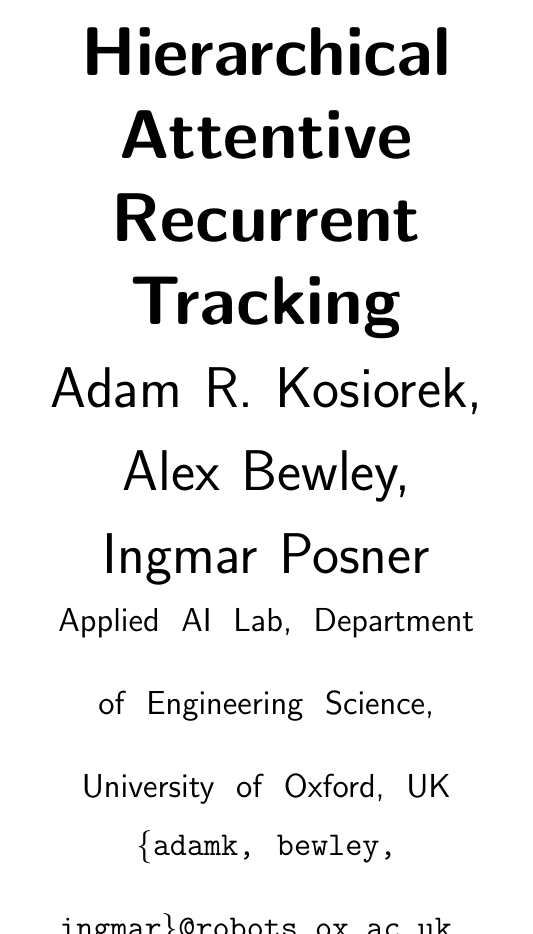
\begin{tikzpicture}
    % Title text
    \node[inner sep=0,text width=0.5\textwidth,text centered,font=\Huge]
%    \node[inner sep=0,
%    text width=0.5\textwidth,
%    text centered,
%    font=\Huge,
%    draw=none,
%    shade,
%    outer color=oriblue,
%    inner color=oriblue] 
    (Title) at (0,0) 
    {
      {\sffamily \Huge \textbf{Hierarchical \mbox{Attentive} Recurrent Tracking}}\\
      {\huge\sffamily Adam R. Kosiorek, Alex Bewley, Ingmar Posner}\\
      \vspace{-0.3\baselineskip}
      {\large\sffamily Applied AI Lab, Department of Engineering Science, University of Oxford, UK}\\
      \vspace{-0.3\baselineskip}
      {\large \texttt{\{adamk, bewley, ingmar\}@robots.ox.ac.uk}}
      \vspace{-0.5\baselineskip}
    };
    % Lab badge
    %\node [mybox] (Lab Badge) at (-1.25, 0) {
     %   \includegraphics[height=\badgeheight]{../badges/a2i_logo.pdf}
    %};
    % University logo
    %\node [mybox] (box) at (0.75, 0) {
     %   \includegraphics[width=0.2\textwidth]{../badges/oxford.pdf}
    %};
\end{tikzpicture}
&
&
\begin{tikzpicture}
% University logo
\node [mybox] (box) at (0, 0) {
	\includegraphics[width=0.2\textwidth]{../badges/oxford.pdf}
};
%\node at (+0.15, 0) {};    
\end{tikzpicture}
\\
\end{tabularx}
\end{center}

%%%%%%%%%%%%%%%%%%%%%%%%%%%%%%%%%%%%%%%%%%%
%
% Spacing between title and main body
%
%%%%%%%%%%%%%%%%%%%%%%%%%%%%%%%%%%%%%%%%%%%

\vspace{1\baselineskip}

%%%%%%%%%%%%%%%%%%%%%%%%%%%%%%%%%%%%%%%%%%%
%
% Columns environment
%
%%%%%%%%%%%%%%%%%%%%%%%%%%%%%%%%%%%%%%%%%%%
\hspace{40mm}

\begin{multicols}{2}

%%%%%%%%%%%%%%%%%%%%%%%%%%%%%%%%%%%%%%%%%%%
%
% Start of content
%
%%%%%%%%%%%%%%%%%%%%%%%%%%%%%%%%%%%%%%%%%%%

\Large

%\input{poster/motivation.tex}
\vspace{2\baselineskip}
\mysection{Problem Statement}

\vspace{1\baselineskip}

\begin{description}[labelsep=1em, leftmargin=!,labelwidth=\widthof{\bfseries Difficulties:},itemsep=.5em]
    \item[What:] Class-agnostic single object tracking in\\ real-world videos with camera motion
    
    \item[Difficulties:] No target-specific discriminative models\\ Cluttered backgrounds with many distractors
    
    \item[How:] Discard uninformative background features\\
                     Learn arbitrary motion models\\
                     Anticipate appearance changes
                     
    \item[Approach:] Recurrent Neural Network with Hierarchical Attention Mechanism
\end{description}
\vspace{1\baselineskip}
\mysection{Hierarchical Attention}

\vspace{1\baselineskip}


    \begin{minipage}[c]{0.3\textwidth}
        \centering
        \begin{subfigure}[b]{1.\textwidth}
            \includegraphics[width=\textwidth]{att_img}
%            \caption*{\textcolor{red}{prediction}, \textcolor{blue}{ground-truth}}
        \end{subfigure}
        
        \hspace{-30pt}
        \begin{minipage}{.9\textwidth}
            \centering
            \vspace{.5em}
            \begin{subfigure}[b]{.31\textwidth}
                \centering
                \includegraphics[width=\textwidth, cfbox=darkgreen 9pt 0pt]{att_glimpse}
                \caption*{\large attention glimpse}
            \end{subfigure}
            \hfill
            \begin{subfigure}[b]{.31\textwidth}
                \centering
                \includegraphics[width=\textwidth, cfbox=white 9pt 0pt]{att_mask}
                \caption*{\large object mask}
            \end{subfigure}
            \hfill
            \begin{subfigure}[b]{.31\textwidth}
                \centering
                \includegraphics[width=\textwidth, cfbox=white 9pt 0pt]{att_overlay}
                \caption*{\large appearance attention}
            \end{subfigure}
            
        \end{minipage}
    \end{minipage}\hfill
    \begin{minipage}[c]{0.3\textwidth}
        \vspace{1\baselineskip}
        \begin{description}[labelsep=1em, leftmargin=!,labelwidth=\widthof{\bfseries Interpretable:}, itemsep=0.5em]
            \item[Bio-inspired:] Two-stream processing pathway and attention mechanisms adapted from human visual cortex.
            \item[Interpretable:] Important features selected by Spatial Attention and Object Segmentation mechanisms.
            \item[Scalable:] Applicable to real-world data due to\\ distractor suppression and auxiliary loss terms.
            \item[Efficient:] Attention quickly discards irrelevant features\\
                              $> 120$ fps on a laptop! 
        \end{description}
    \end{minipage}

%    \item[Why:] Attention Mechanisms adapted from Human Visual Cortex suppress distractors and increase efficiency 
%\item[Result:] Interpretable Neural Tracker applicable to Real-World Data 

\vspace{1\baselineskip}

%\newpage

\mysection{Two-Stream Attentive Model}

\vspace{.5\baselineskip}

\begin{minipage}[c]{0.3\textwidth}
    \centering
    \begin{minipage}[c]{\textwidth}
    \includegraphics[width=\textwidth]{arch.pdf}
    \end{minipage}
    \vspace{-1\baselineskip}
    
    \begin{minipage}[c]{0.5\textwidth}
        \begin{description}[labelsep=1em, leftmargin=!,labelwidth=\widthof{\bfseries $\bmapt$}]
            \item[$\bxt$] input image
            \item[$\bgt$] attention glimpse
            \item[$\bmapt$] appearance-based features
            \item[$\bst$] object segmentation
            \item[$\bvt$] masked features
        \end{description}
    \end{minipage}\hfill
    \begin{minipage}[c]{0.5\textwidth}
       \begin{description}[labelsep=1em, leftmargin=!,labelwidth=\widthof{\bfseries $\Delta \widehat{\bb}_t$}]
            \item[$\B{h}_t$] hidden state
            \item[$\bot$] LSTM output
            \item[$\bapp_{t+1}$] appearance
            \item[$\Delta \widehat{\bb}_t$] bounding-box update
            \item[$\ba_{t+1}$] spatial attention
        \end{description}
    \end{minipage}
\end{minipage}
\begin{minipage}{0.3\textwidth}
   \vspace{1em}
   \caption*{\Large \B{Appearance attention architecture}:}
%   \vspace{.5em}
   \begin{minipage}[c]{0.5\textwidth}
       \centering
       \includegraphics[width=\textwidth]{impl.pdf}
   \end{minipage}\hfill
    \begin{minipage}{0.6\textwidth}
%    \begin{description}[leftmargin=\parindent]
%%        \item[V1] shared CNN
%        \item[Dorsal Stream] Dynamic\\ Filter Network (DFN)\\ conditioned on appearance
%%        \item[Ventral Stream] CNN
%    \end{description}
    \B{Dorsal Stream:} Dynamic Filter\\ Network [4] conditioned on appearance\\ finds target-specific features
    \end{minipage}
\vspace{.5em}
\end{minipage}
\begin{minipage}{0.3\textwidth}
    \centering
       \begin{minipage}[c]{0.26\textwidth}
        \B{V1:} Shared~CNN
    \end{minipage}
    \begin{minipage}[c]{0.71\textwidth}
        \B{Ventral Stream:} CNN extracts visual features
    \end{minipage}
\end{minipage}

\vspace{\baselineskip}
%\input{poster/method.tex}

%\vspace{0\baselineskip}


\newpage


\mysection{Learning to Attend for Tracking}



The model is optimised for the following three objectives.
\begin{description}[leftmargin=\parindent,labelsep=1em]
	
	\item[Main Tracking Objective:] Maximise the overlap of predicted box with the true object.
	
	\item[Spatial Attention:] The glimpse should contain the object, but shouldn't be too big.
	
	\item[Appearance Attention:] The dynamic appearance features should respond specifically to the target object.
	
	
\end{description}


\vspace{.5\baselineskip}
\centering
\begin{minipage}[c]{.4\textwidth}
    \centering
    \includegraphics[width=\textwidth]{soft_id_swap}
%    \vspace{.2\baselineskip}
    \caption*{\large Appearance attention loss (top) prevents an ID swap when a pedestrian is occluded by another one (bottom).}
\end{minipage}
\begin{minipage}[c]{.4\textwidth}
    \centering
%    \vspace{.5\baselineskip}
    \includegraphics[width=\textwidth]{soft_att}
%    \vspace{.1\baselineskip}
   \caption*{\large Left to right: glimpses and segmentations learned with and without appearance loss.
   Attention loss leads to distractor suppression.} 
\end{minipage}


%\mysection{Loss}
\vspace{.5\baselineskip}
    \centering
    Directly optimise Intersection-over-Union (IoU) and guide attention mechanisms.
%\begin{equation*}
%\loss[\mathrm{HART}]{\cdot} = \lambda_{\mathrm{t}} \loss[\mathrm{t}]{\cdot} + \lambda_{\mathrm{s}} \loss[\mathrm{s}]{\cdot} + \lambda_{\mathrm{a}} \loss[\mathrm{a}]{\cdot}  + \reg{ \B{\lambda} } + \beta \reg{ \cdot }
%\end{equation*}
\begin{equation*}
\loss[\mathrm{HART}]{\cdot} = \lambda_{\mathrm{t}} \loss[\mathrm{t}]{\cdot} + \lambda_{\mathrm{s}} \loss[\mathrm{s}]{\cdot} + \lambda_{\mathrm{a}} \loss[\mathrm{a}]{\cdot} + \beta \reg{ \cdot }
\end{equation*}

\begin{description}[leftmargin=\parindent,labelsep=1em]

\item[Tracking:] Negative log of Intersection-over-Union.
\begin{equation*}
    \loss[\mathrm{t}]{\data, \theta} = \expc[\p{\widehat{\bb}_{1:T}}{\bxTs, \bb_1}]{ -\log \mathrm{IoU} \fences{\widehat{\bb}_t, \bbt}}
\end{equation*}

\item[Spatial Attention:] It follows the object, but shouldn't be too big.
\begin{equation*}
    \loss[\mathrm{s}]{\data, \theta} = \expc[\p{\baTs}{\bxTs, \bb_1}]{ -\log \fences*{\frac{ \bat \cap \bbt }{\mathrm{area}\fences{\bbt}} } -\log \fences { 1 - \mathrm{IoU} \fences{\bat, \bxt} } }
\end{equation*}

\item[Appearance Attention:] Cross-entropy with dynamically created target mask $\tau \fences { \bat, \bbt }$:
$\loss[\mathrm{a}]{\data, \theta} =   \expc[\p{\baTs, \bsTs}{\bxTs, \bb_1}]{ H \fences{ \tau \fences { \bat, \bbt }, \bst  } }$.



\begin{minipage}[c]{.3\textwidth}
    \centering
    \vspace{0.75em}
    \caption*{\large With Appearance Attention Loss: Successful Tracking}
    \includegraphics[width=\textwidth]{soft_id_swap}
    \caption*{\large Without Appearance Attention Loss: ID Swap}
\end{minipage}
\end{description}





\mysection{Pedestrian Tracking: KTH Dataset [2]}

\vspace{1\baselineskip}

\begin{minipage}[c]{0.45\textwidth}
    \centering
    \vspace{-1.5em}
    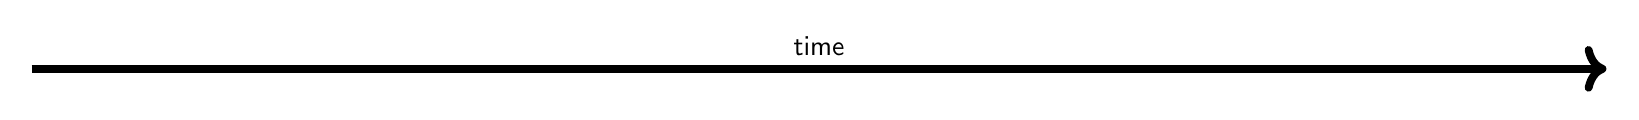
\begin{tikzpicture}
    \draw[line width=1mm, ->] (-10, 0) -- node[above] {time} (10, 0);
    \end{tikzpicture}
    \includegraphics[width=\textwidth]{kth_overlay_16}
    
    \begin{minipage}[c]{0.55\textwidth}
        \begin{itemize}
            \item Attention, prediction and ground-truth overlap at initialization.
            \item Every $16^{th}$ frame of the\\ sequence at 25 fps.
            \item $2^{nd}$ row: attention glimpses multiplied with appearance attention.
        \end{itemize}
    \end{minipage}\hfill   
    {\Large
    \begin{minipage}[c]{0.45\textwidth}
    	\hspace{.9em}
        \begin{tabular}{c|c}
            \multicolumn{2}{c}{Intersection over Union}\\
            Kahou \emph{et. al.} [1] & Ours\\
            \midrule
            0.55 & \B{0.77}
        \end{tabular}
    \end{minipage}
}
    \vspace{.5em}
\end{minipage}



%\vspace{0\baselineskip}

\mysection{Scaling to Real-World Data: KITTI [3]}

\vspace{0.5\baselineskip}

    \begin{minipage}[c]{0.45\textwidth}
        \centering
        % \todo[inline]{other results are on their way}
        \includegraphics[width=\textwidth]{kitti_iou_fig}
        
        \hspace{-1.55em}
        {\large
        \begin{minipage}[c]{0.5\linewidth}
            \centering
            \begin{tabular}{c|c|c|c}
                \multicolumn{4}{c}{Average IoU on KITTI over 60 time-steps}\\
                Kahou \emph{et. al.} [1] & Spatial Att & App Att & \B{HART}\\
                \midrule
                0.14 & 0.60 & 0.78 & \B{0.81}
            \end{tabular}
        \caption*{\large Spatial Att - no appearance attention\\ App Att - no appearance attention loss}
        \end{minipage}
        }\hfill
        \begin{minipage}[c]{0.425\linewidth}
            \vspace{.3em}
            IoU curves on KITTI over 60 time-steps; HART~(train) presents evaluation on the train set.
        \end{minipage}
    \end{minipage}
   
    \vspace{0.25em}

%\mysection{Conclusion}

\begin{description}[labelsep=1em, leftmargin=!,labelwidth=\widthof{\bfseries Interpretable:}]
    \item[Bio-inspired:] Neural Recurrent tracking with\\ Attention Mechanisms.
    \item[Interpretable:] Important features selected by spatial attention and object segmentation mechanisms.
    \item[Scalable:] Auxiliary loss terms allow scaling to\\ complex real-world datasets.
    \item[Efficient:] $> 120$ fps on a laptop! 
    \item[Future Work:] Multi-object tracking.
\end{description}

\vspace{-2mm}


\vspace{.5\baselineskip}

%{\Large References:}
\mysection{References}
{\large
\begin{description}
    \item[[1]] Samira Ebrahimi Kahoú, Vincent Michalski, and Roland Memisevic. RATM: Recurrent Attentive Tracking Model. CVPR Workshop, 2017.
    \item[[2]] Christian Schuldt, Ivan Laptev, and Barbara Caputo. Recognizing human actions: A local SVM approach. ICPR. IEEE, 2004.
    \item[[3]] A. Geiger, P. Lenz, C. Stiller, and R. Urtasun. Vision meets robotics: The KITTI dataset. IJRR,
    32(11):1231–1237, 2013.
    \item [[4]] Bert De Brabandere, Xu Jia, Tinne Tuytelaars, and Luc Van Gool. Dynamic Filter Networks. NIPS, 2016.
\end{description}
}
%\vspace{0.5\baselineskip}
{\large \faGithub\ \url{https://github.com/akosiorek/hart} \\ \faYoutube\ \url{https://youtu.be/Vvkjm0FRGSs}}

\end{multicols}


\end{poster}

\end{document}
